\documentclass[11pt]{article}
\usepackage[textwidth=18.0cm, textheight=23.0cm, top=2.0cm]{geometry}
\usepackage{pst-all}
\usepackage{amssymb}
\usepackage{tikz}
\usepackage{underscore}\begin{document}
\pagestyle{empty}


ClassName: \underline{\textbf{Class_01.2bp-2}}
\par
BinSize: \underline{\textbf{10 × 10}}
\par
ReduceSize: \underline{\textbf{10 × 10}}
\par
TypeNum: \underline{\textbf{20}}
\par
Num: \underline{\textbf{20}}
\par
OutS: \underline{\textbf{900}}
\par
InS: \underline{\textbf{650}}
\par
Rate: \underline{\textbf{0.722}}
\par
UB: \underline{\textbf{9}}
\par
LB0: \underline{\textbf{8}}
\par
LB: \underline{\textbf{8}}
\par
LBWithCut: \underline{\textbf{9}}
\par
NodeCut: \underline{\textbf{1}}
\par
ExtendedNodeCnt: \underline{\textbf{1}}
\par
GenNodeCnt: \underline{\textbf{1}}
\par
PrimalNode: \underline{\textbf{0}}
\par
ColumnCount: \underline{\textbf{24}}
\par
TotalCutCount: \underline{\textbf{9}}
\par
RootCutCount: \underline{\textbf{9}}
\par
LPSolverCnt: \underline{\textbf{17}}
\par
PricingSolverCnt: \underline{\textbf{17}}
\par
BranchAndBoundNum: \underline{\textbf{1}}
\par
isOpt: \underline{\textbf{true}}
\par
TimeOnPrimal: \underline{\textbf{0.000 s}}
\par
TimeOnPricing: \underline{\textbf{0.531 s}}
\par
TimeOnRmp: \underline{\textbf{0.063 s}}
\par
TotalTime: \underline{\textbf{0.672 s}}
\par
\newpage



\begin{tikzpicture}[shorten >=1pt,scale=1.0,every node/.style={scale=1.0},->]
\tikzstyle{vertex}=[circle,fill=black!25,minimum size=14pt,inner sep=0pt]
\filldraw[fill=gray!40!white, draw=black] (0,0) rectangle (15.0,15.0);
\foreach \name/\x/\y/\w/\h in {10x9/0.0/0.0/15.0/13.5}
\filldraw[fill=white!40!white, draw=black] (\x,\y) rectangle node[draw] (\name) {\name} ++(\w,\h);
\end{tikzpicture}


w =10 , h =9 , x =0 , y =0 , v =90
\par
\newpage


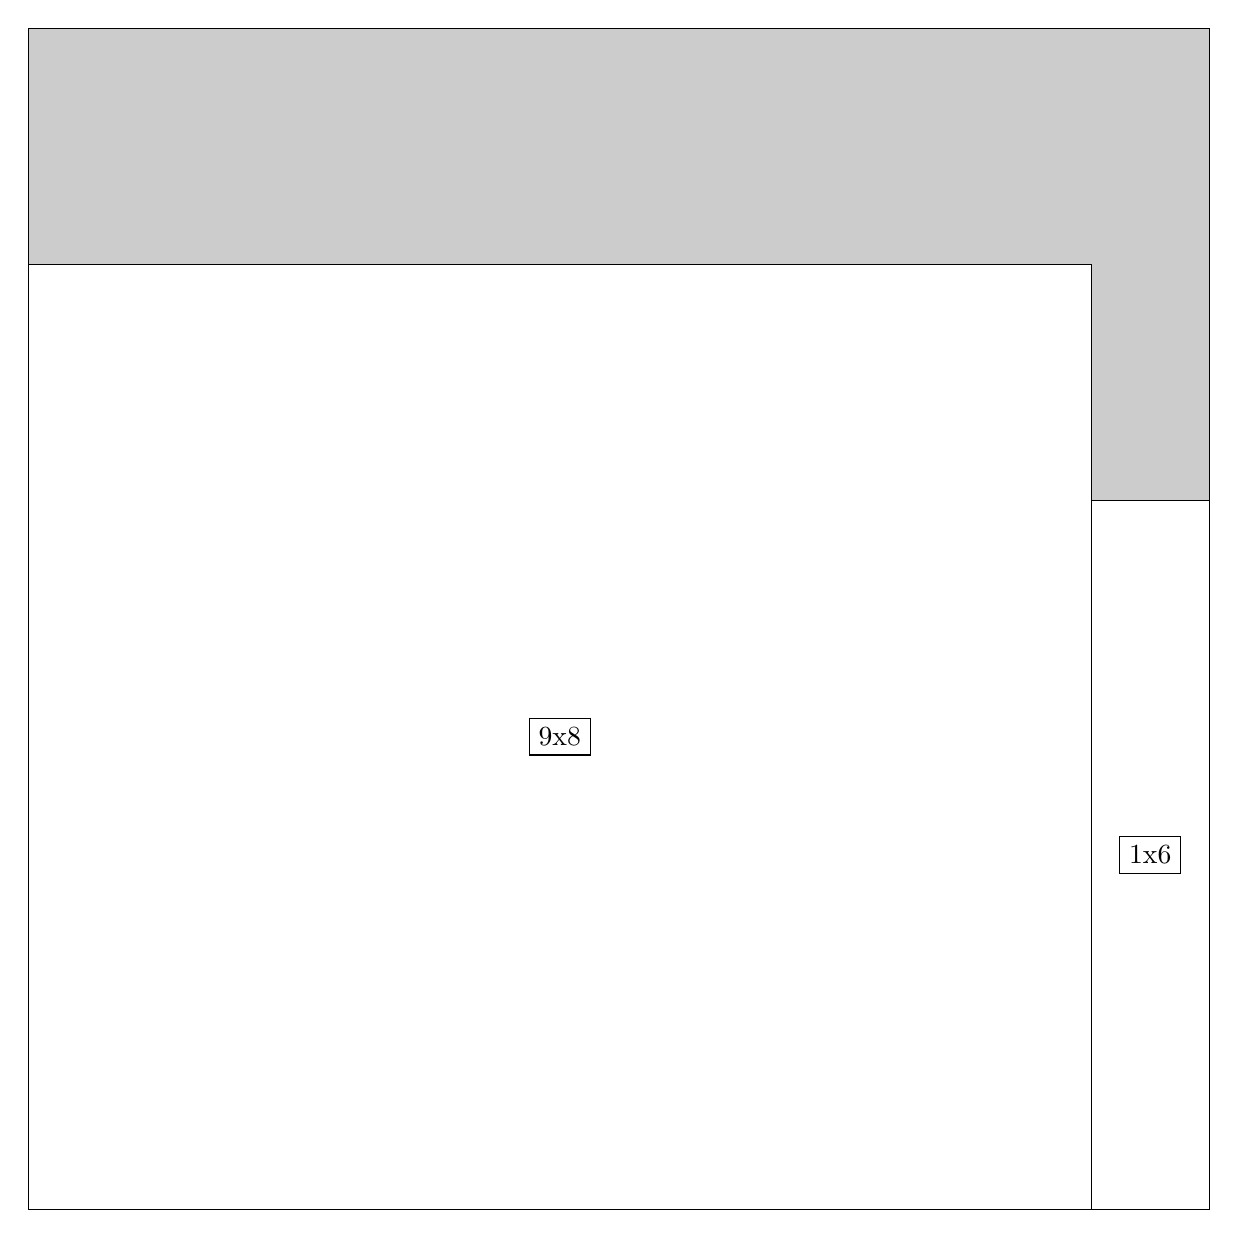
\begin{tikzpicture}[shorten >=1pt,scale=1.0,every node/.style={scale=1.0},->]
\tikzstyle{vertex}=[circle,fill=black!25,minimum size=14pt,inner sep=0pt]
\filldraw[fill=gray!40!white, draw=black] (0,0) rectangle (15.0,15.0);
\foreach \name/\x/\y/\w/\h in {9x8/0.0/0.0/13.5/12.0,1x6/13.5/0.0/1.5/9.0}
\filldraw[fill=white!40!white, draw=black] (\x,\y) rectangle node[draw] (\name) {\name} ++(\w,\h);
\end{tikzpicture}


w =9 , h =8 , x =0 , y =0 , v =72
\par
w =1 , h =6 , x =9 , y =0 , v =6
\par
\newpage


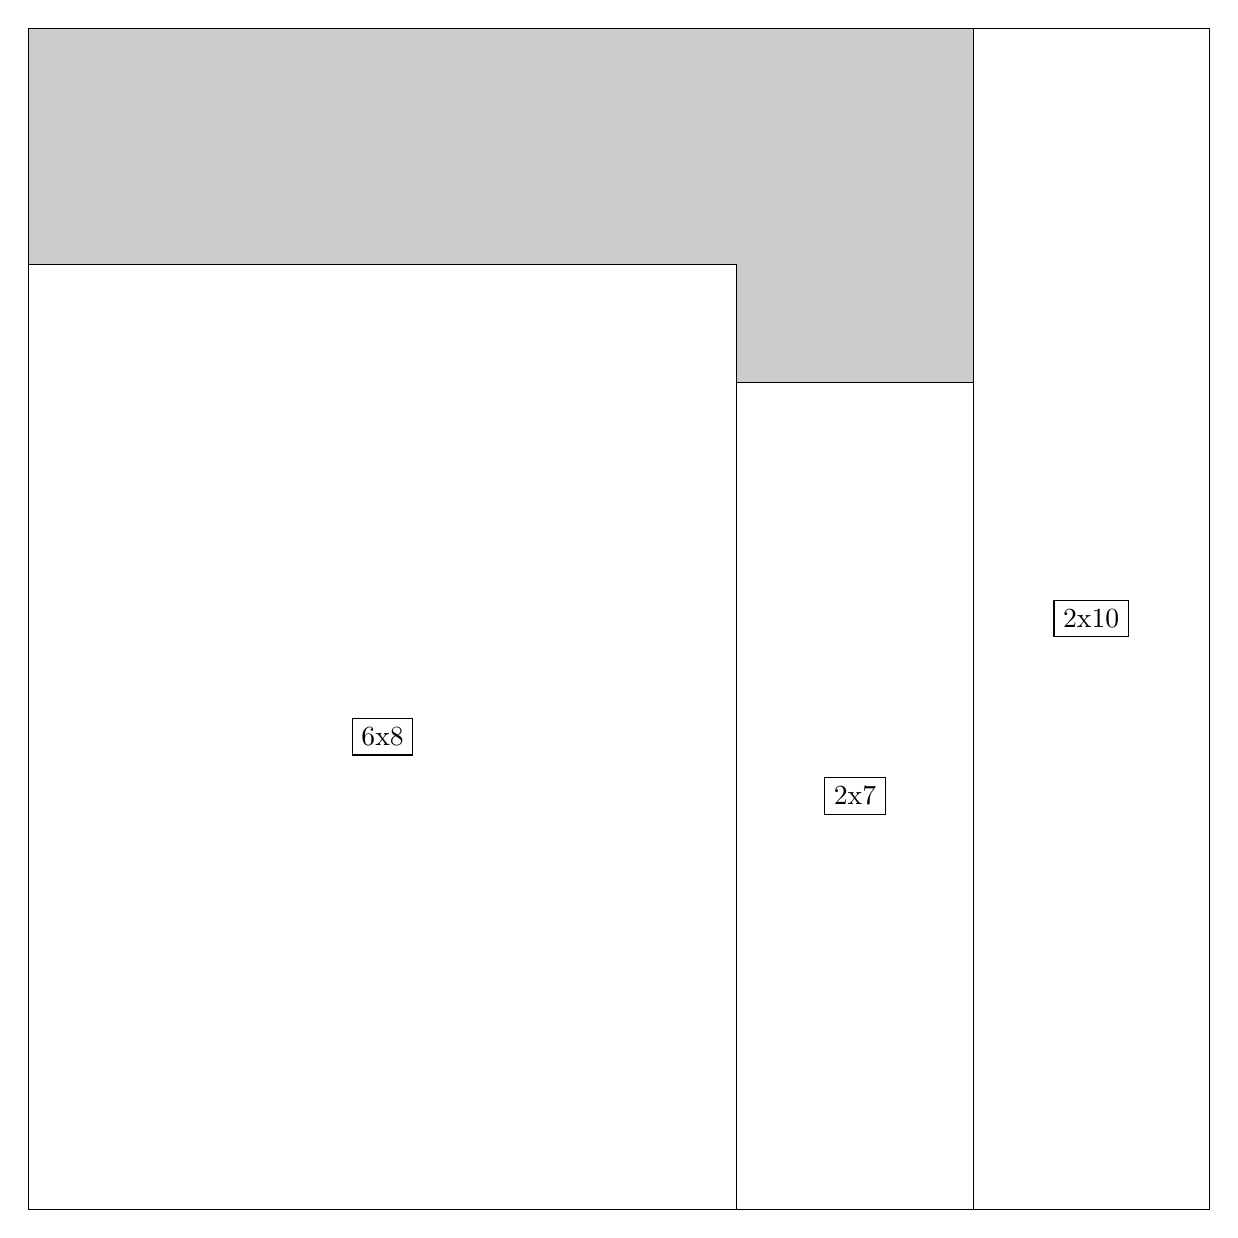
\begin{tikzpicture}[shorten >=1pt,scale=1.0,every node/.style={scale=1.0},->]
\tikzstyle{vertex}=[circle,fill=black!25,minimum size=14pt,inner sep=0pt]
\filldraw[fill=gray!40!white, draw=black] (0,0) rectangle (15.0,15.0);
\foreach \name/\x/\y/\w/\h in {6x8/0.0/0.0/9.0/12.0,2x10/12.0/0.0/3.0/15.0,2x7/9.0/0.0/3.0/10.5}
\filldraw[fill=white!40!white, draw=black] (\x,\y) rectangle node[draw] (\name) {\name} ++(\w,\h);
\end{tikzpicture}


w =6 , h =8 , x =0 , y =0 , v =48
\par
w =2 , h =10 , x =8 , y =0 , v =20
\par
w =2 , h =7 , x =6 , y =0 , v =14
\par
\newpage


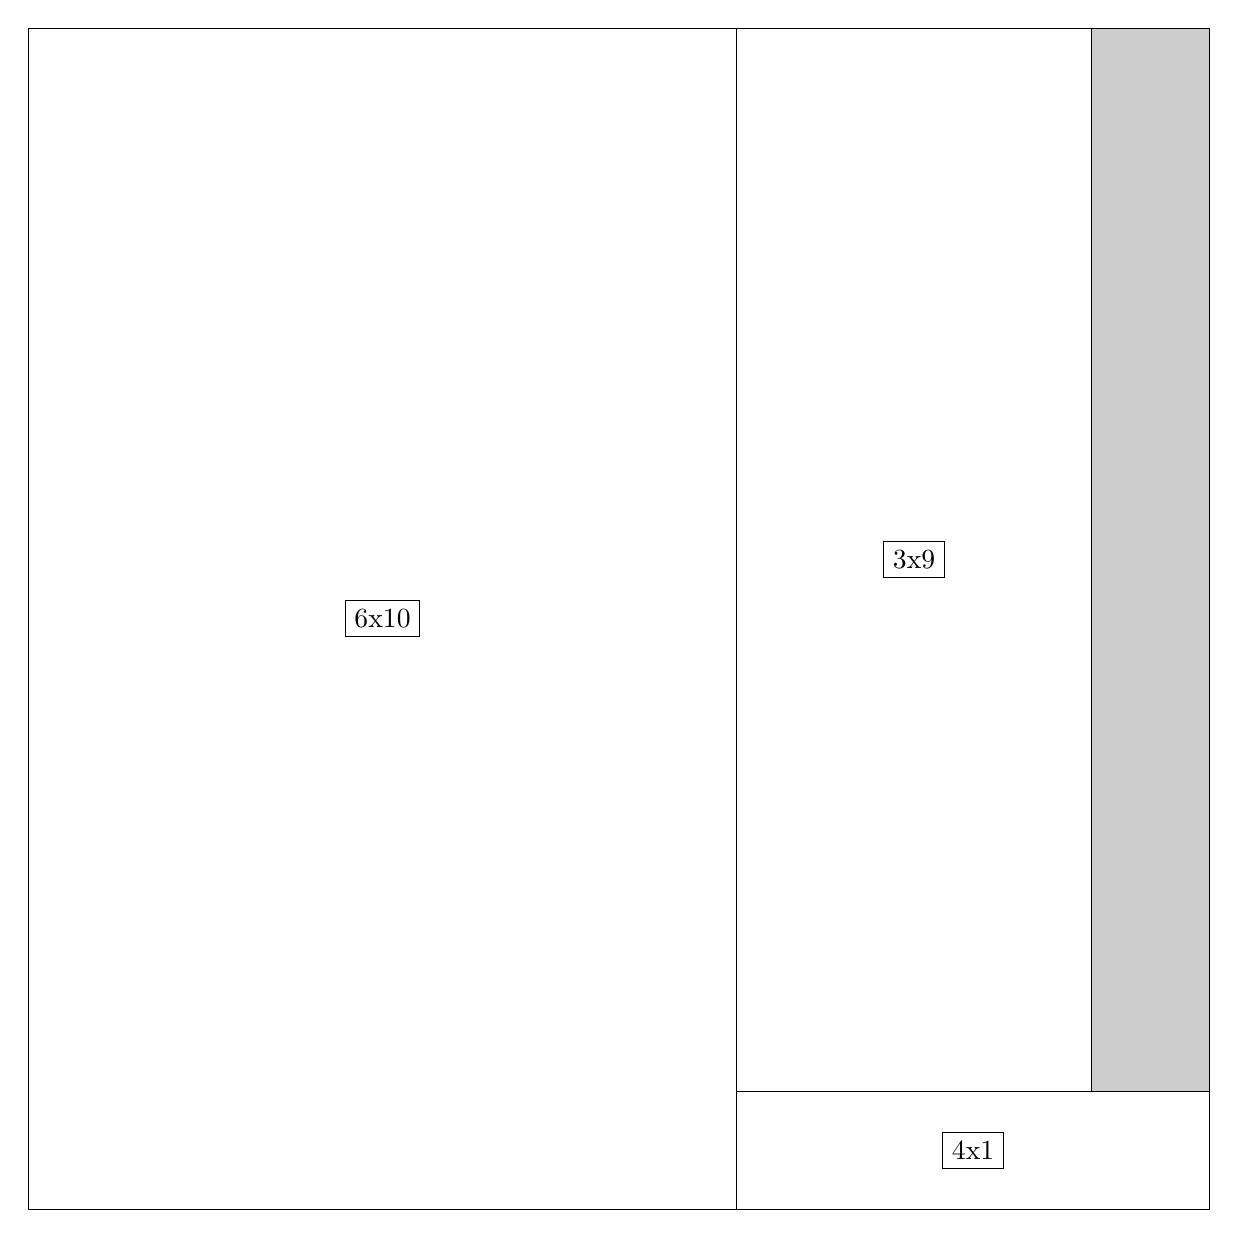
\begin{tikzpicture}[shorten >=1pt,scale=1.0,every node/.style={scale=1.0},->]
\tikzstyle{vertex}=[circle,fill=black!25,minimum size=14pt,inner sep=0pt]
\filldraw[fill=gray!40!white, draw=black] (0,0) rectangle (15.0,15.0);
\foreach \name/\x/\y/\w/\h in {3x9/9.0/1.5/4.5/13.5,6x10/0.0/0.0/9.0/15.0,4x1/9.0/0.0/6.0/1.5}
\filldraw[fill=white!40!white, draw=black] (\x,\y) rectangle node[draw] (\name) {\name} ++(\w,\h);
\end{tikzpicture}


w =3 , h =9 , x =6 , y =1 , v =27
\par
w =6 , h =10 , x =0 , y =0 , v =60
\par
w =4 , h =1 , x =6 , y =0 , v =4
\par
\newpage


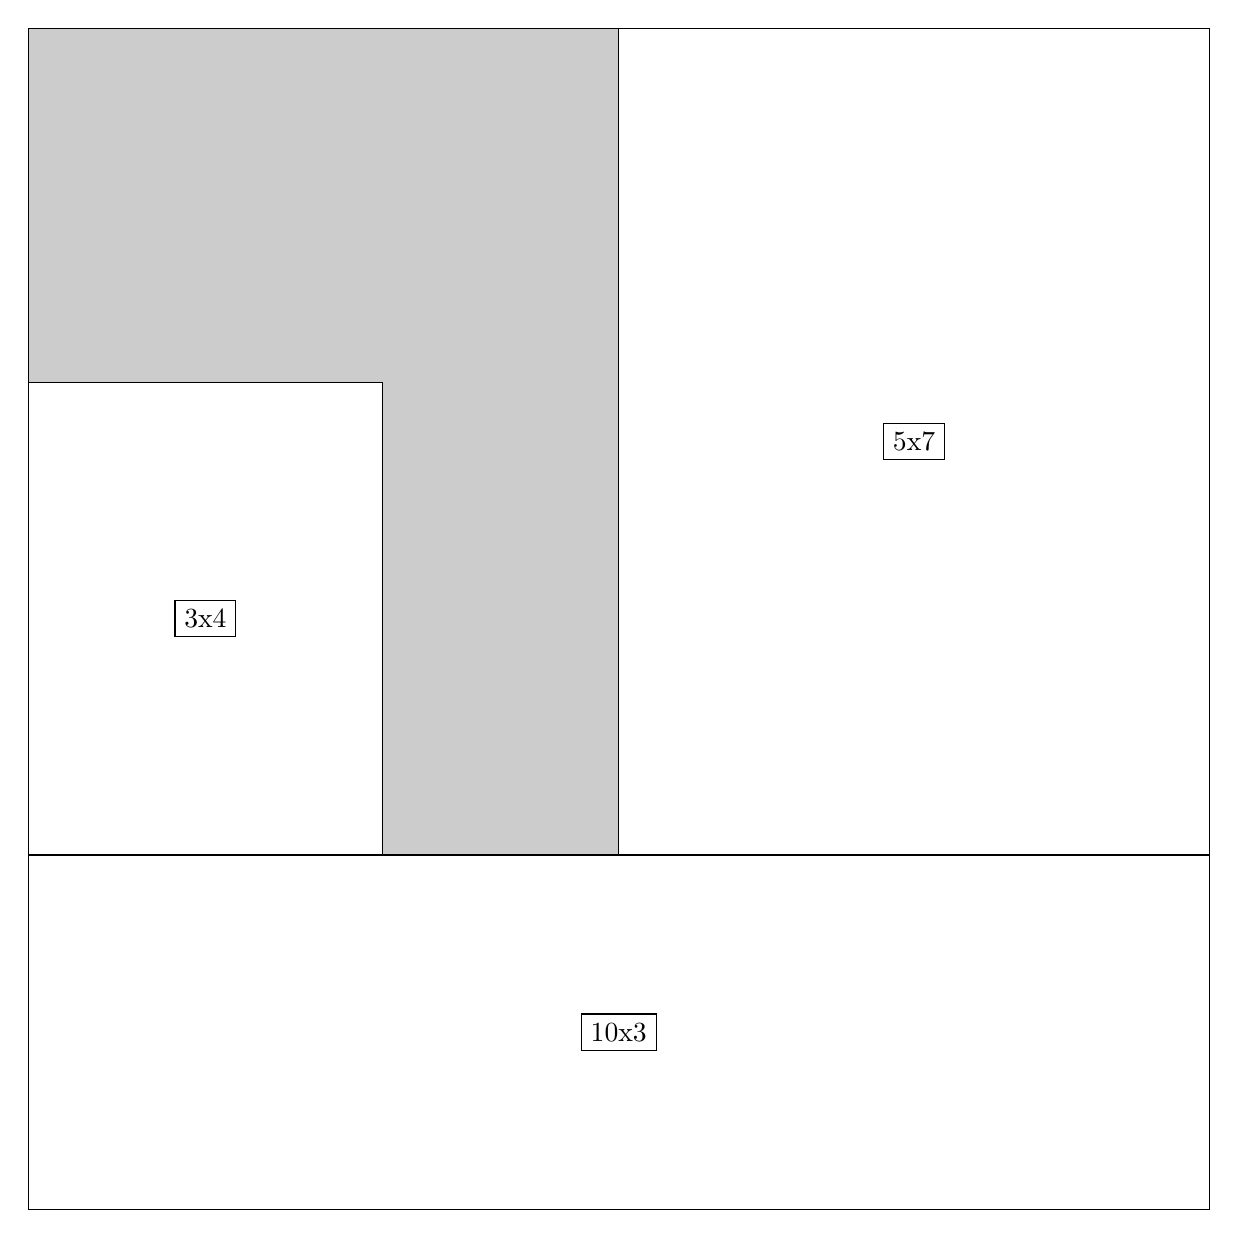
\begin{tikzpicture}[shorten >=1pt,scale=1.0,every node/.style={scale=1.0},->]
\tikzstyle{vertex}=[circle,fill=black!25,minimum size=14pt,inner sep=0pt]
\filldraw[fill=gray!40!white, draw=black] (0,0) rectangle (15.0,15.0);
\foreach \name/\x/\y/\w/\h in {3x4/0.0/4.5/4.5/6.0,5x7/7.5/4.5/7.5/10.5,10x3/0.0/0.0/15.0/4.5}
\filldraw[fill=white!40!white, draw=black] (\x,\y) rectangle node[draw] (\name) {\name} ++(\w,\h);
\end{tikzpicture}


w =3 , h =4 , x =0 , y =3 , v =12
\par
w =5 , h =7 , x =5 , y =3 , v =35
\par
w =10 , h =3 , x =0 , y =0 , v =30
\par
\newpage


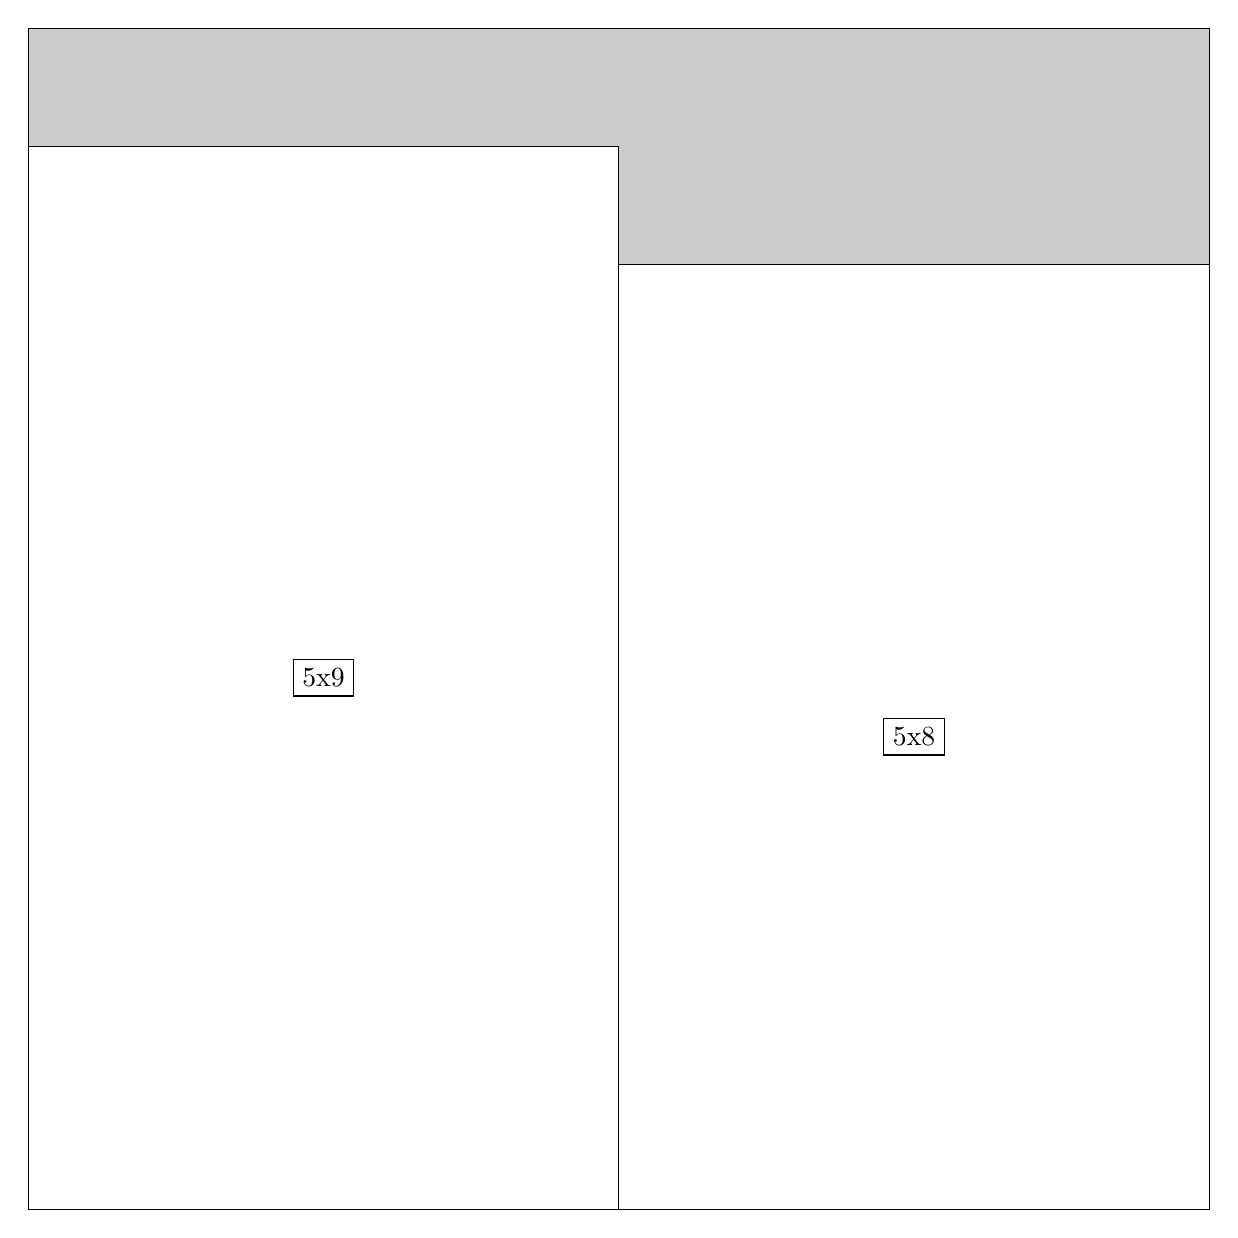
\begin{tikzpicture}[shorten >=1pt,scale=1.0,every node/.style={scale=1.0},->]
\tikzstyle{vertex}=[circle,fill=black!25,minimum size=14pt,inner sep=0pt]
\filldraw[fill=gray!40!white, draw=black] (0,0) rectangle (15.0,15.0);
\foreach \name/\x/\y/\w/\h in {5x9/0.0/0.0/7.5/13.5,5x8/7.5/0.0/7.5/12.0}
\filldraw[fill=white!40!white, draw=black] (\x,\y) rectangle node[draw] (\name) {\name} ++(\w,\h);
\end{tikzpicture}


w =5 , h =9 , x =0 , y =0 , v =45
\par
w =5 , h =8 , x =5 , y =0 , v =40
\par
\newpage


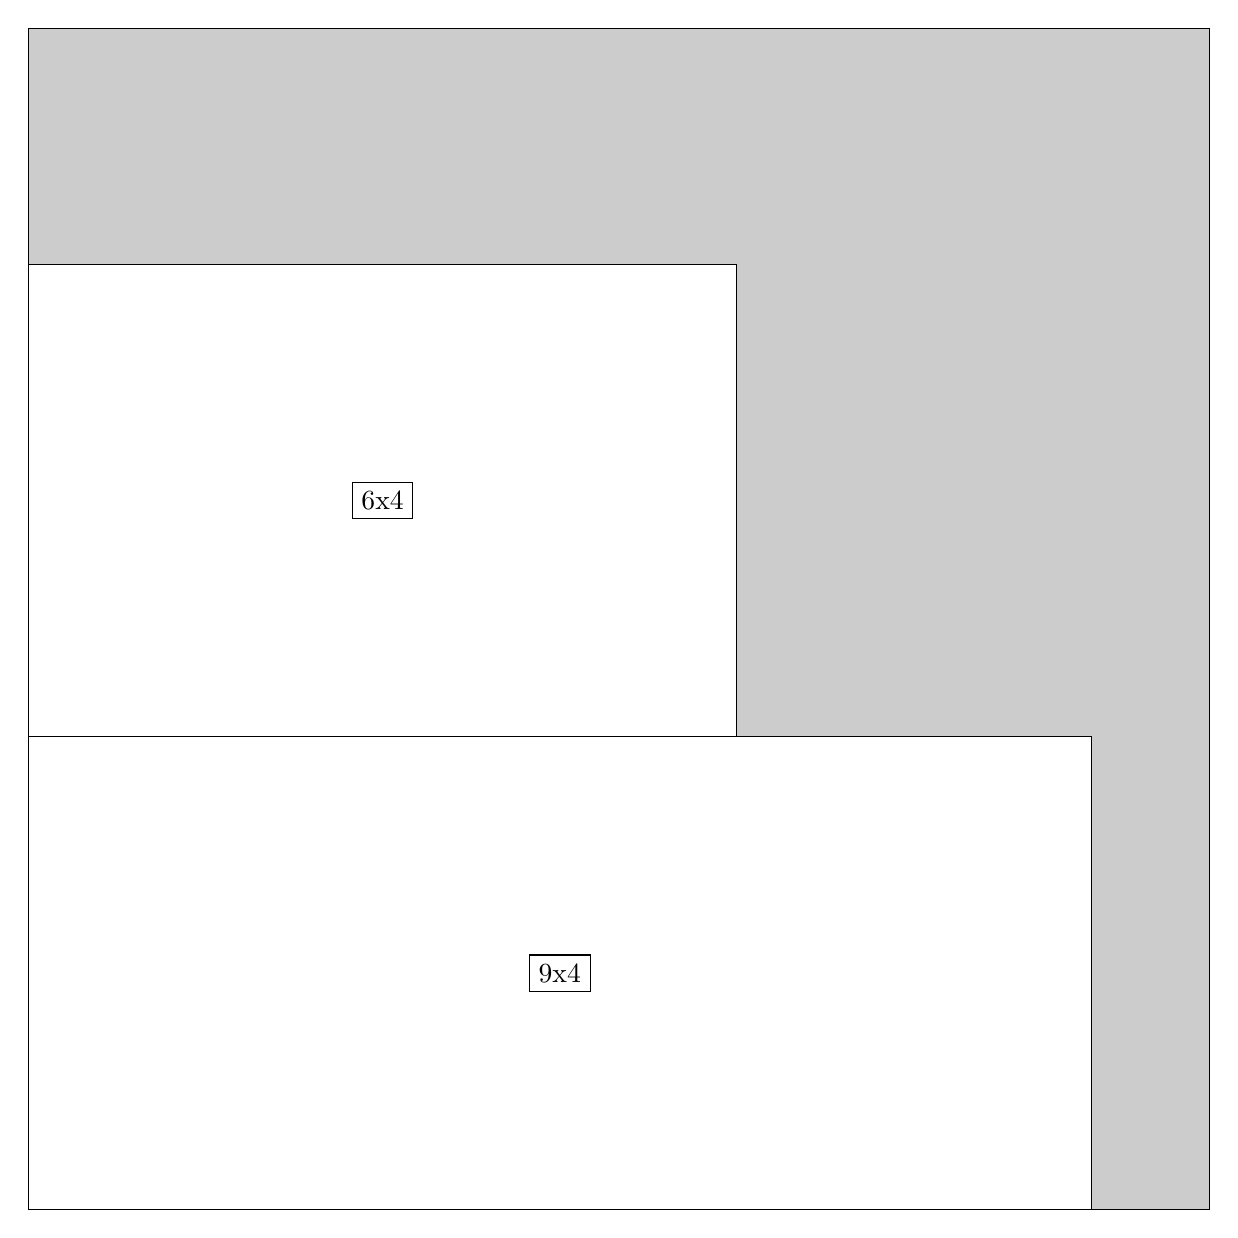
\begin{tikzpicture}[shorten >=1pt,scale=1.0,every node/.style={scale=1.0},->]
\tikzstyle{vertex}=[circle,fill=black!25,minimum size=14pt,inner sep=0pt]
\filldraw[fill=gray!40!white, draw=black] (0,0) rectangle (15.0,15.0);
\foreach \name/\x/\y/\w/\h in {9x4/0.0/0.0/13.5/6.0,6x4/0.0/6.0/9.0/6.0}
\filldraw[fill=white!40!white, draw=black] (\x,\y) rectangle node[draw] (\name) {\name} ++(\w,\h);
\end{tikzpicture}


w =9 , h =4 , x =0 , y =0 , v =36
\par
w =6 , h =4 , x =0 , y =4 , v =24
\par
\newpage


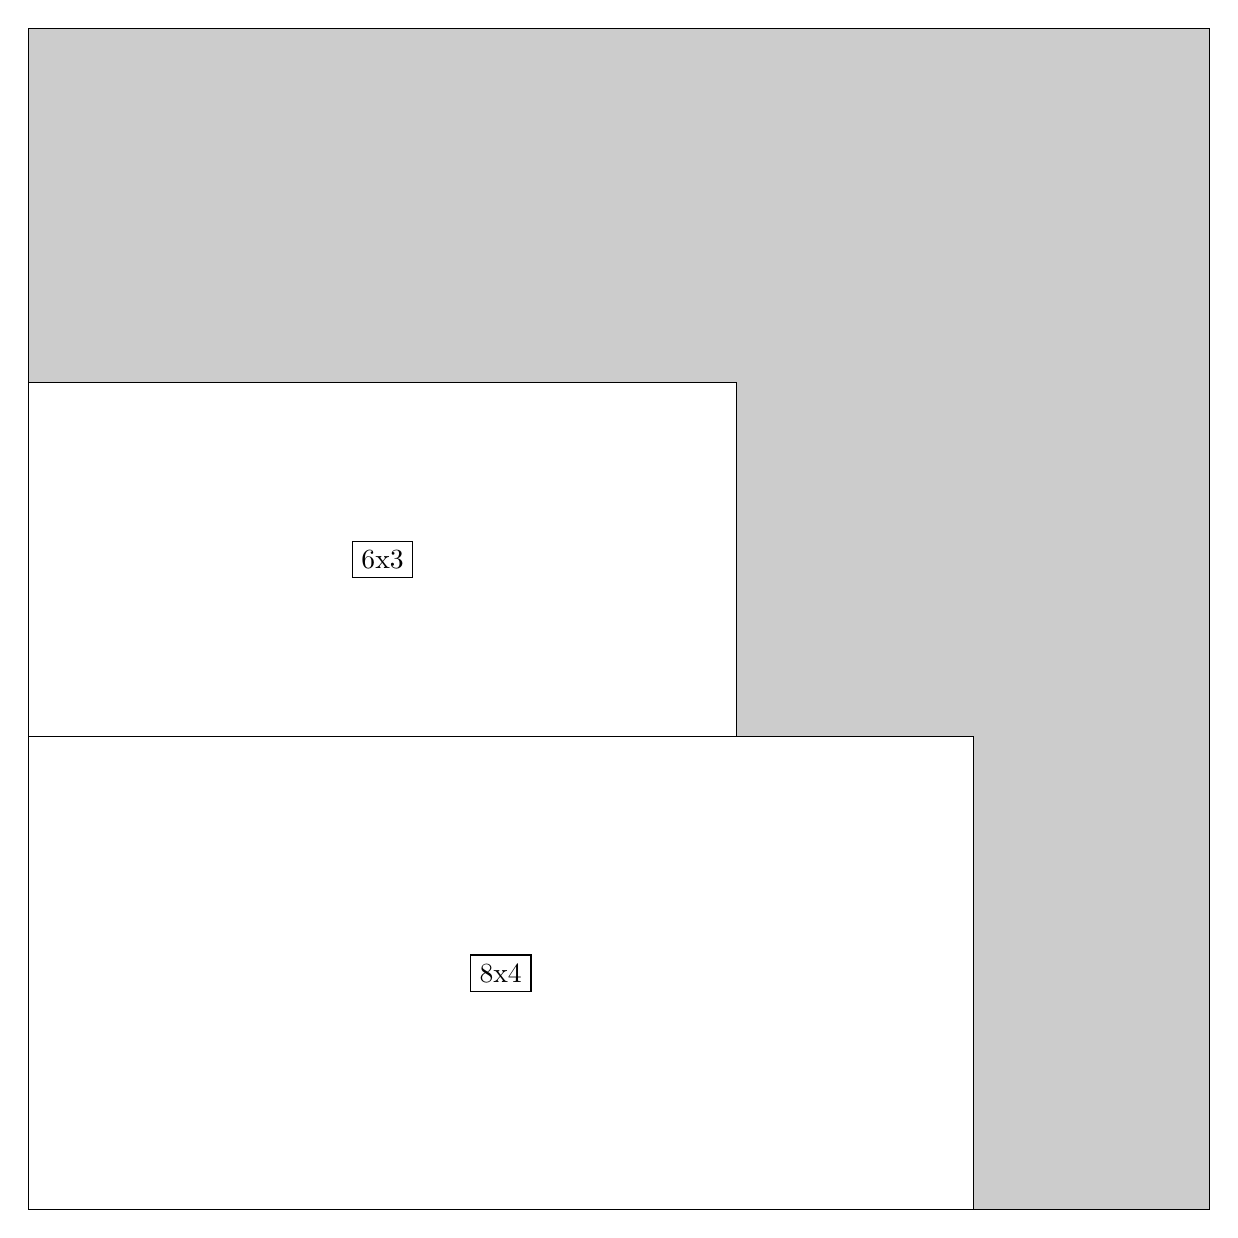
\begin{tikzpicture}[shorten >=1pt,scale=1.0,every node/.style={scale=1.0},->]
\tikzstyle{vertex}=[circle,fill=black!25,minimum size=14pt,inner sep=0pt]
\filldraw[fill=gray!40!white, draw=black] (0,0) rectangle (15.0,15.0);
\foreach \name/\x/\y/\w/\h in {8x4/0.0/0.0/12.0/6.0,6x3/0.0/6.0/9.0/4.5}
\filldraw[fill=white!40!white, draw=black] (\x,\y) rectangle node[draw] (\name) {\name} ++(\w,\h);
\end{tikzpicture}


w =8 , h =4 , x =0 , y =0 , v =32
\par
w =6 , h =3 , x =0 , y =4 , v =18
\par
\newpage


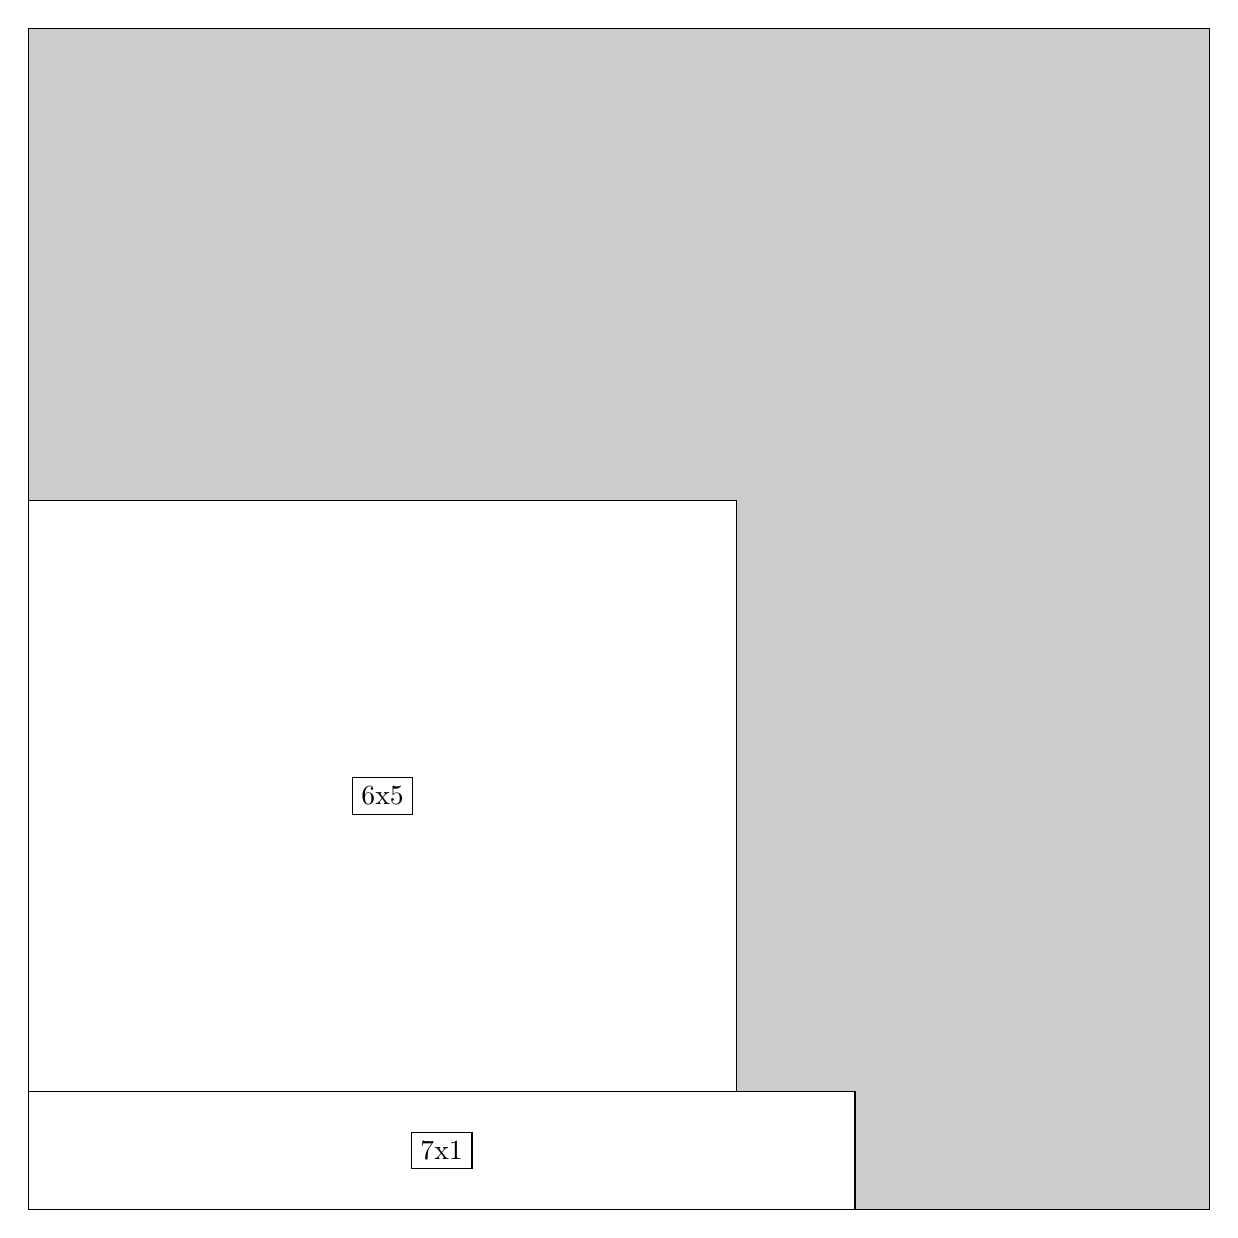
\begin{tikzpicture}[shorten >=1pt,scale=1.0,every node/.style={scale=1.0},->]
\tikzstyle{vertex}=[circle,fill=black!25,minimum size=14pt,inner sep=0pt]
\filldraw[fill=gray!40!white, draw=black] (0,0) rectangle (15.0,15.0);
\foreach \name/\x/\y/\w/\h in {6x5/0.0/1.5/9.0/7.5,7x1/0.0/0.0/10.5/1.5}
\filldraw[fill=white!40!white, draw=black] (\x,\y) rectangle node[draw] (\name) {\name} ++(\w,\h);
\end{tikzpicture}


w =6 , h =5 , x =0 , y =1 , v =30
\par
w =7 , h =1 , x =0 , y =0 , v =7
\par
\newpage


\end{document}